% \documentclass[10pt, oneside, english]{article}   	
\documentclass[10pt, oneside]{article}
\usepackage{geometry}                		
\geometry{a4paper}                   		
% \usepackage[english, es-noindentfirst]{babel}
% \selectlanguage{english}
\usepackage[utf8]{inputenc}               		
\usepackage{graphicx}			
\usepackage{amssymb}
\usepackage{authblk}
\usepackage{multicol}
\usepackage{rotating}


\title{Word embeddings for predicting political affiliation based on Twitter data}

\author[]{Ibrahim Abdelaziz}
\author[]{Oliver Berg}
\author[]{Angjela Davitkova}
\author[]{Venkatesh Iyer}
\author[]{Shriram Selvakumar}
\author[]{Kumar Shridhar}
\author[]{Saurabh Varshneya}
\affil[1]{Technische Universität Kaiserslautern}

\date{\today}


\begin{document}
\maketitle
\begin{multicols}{2}


\section{Abstract}

Twitter as one of today's biggest social media platforms allows political figures to express their thinking easily and with a concise message. We propose a generic way of classifying political affiliation based on Twitter posts. This involves Word2Vec vector representations of the input data and utilizes pretrained embeddings for the German language. With this we have shown to be capable of insightfully position German political figures in the political spectrum. 


\section{Introduction}

Social media platforms like \emph{Twitter} allows people of interest to communicate their personal opinion, and as such e.g. indicating political alignment, through a comprised message being only a few hundred character long. This yields broad potential to characterize personality traits such as political affiliation on.

Generally speaking, political motives were shown to be consistently predictable with an accuracy better than chance already \cite{Biessmann2017}. Today, sentiment classification is mostly done using recurrent- or convolutional neural networks \cite{Kim2014}. In connection to the given focus of working on Twitter data, \cite{Cohen2013} introduces interesting questions concerning applicability of classification onto real data outside the training samples.

This paper therefore proposes a \emph{deep learning} based classification model together with \emph{word embeddings} \cite{Pelevinala2016}. This allows a later \emph{quantitative analysis} to find interesting constellations within the (German) political spectrum.
We leverage word embeddings to represent words in context. We thereby restrict ourselves to pretrained models. Subsequently, a convolutional neural network (CNN) holistically classifies the Twitter profile by assigning each Twitter message a separate party label and combining these into a complete class score.  


\section{Datasets and Feature Extraction} 

The dataset used in this approach was constructed of German politicians' Tweets posted on their Twitter accounts, retrieved from the website “https://www.wahl.de/”, which includes around 1000 German politicians' profiles. Politician’s name, political party, and Twitter username were gathered for each profile.
 
The retrieved Twitter accounts were also filtered to include only those belonging to the seven major political parties, namely "CDU", "CSU", SPD", "FDP", "GRÜNE", "LINKE" and "AFD", ordered by age of introduction into German parliament (old to new). 

After the filtering stage this leaves a list of around 700 politicians, for which up to 1000 of the most recent Tweets are  gathered using the Twitter API. Since some parties do have greater number of Tweets compared to other parties and to create a balanced set for training our model, we used restricted ourselves to at most 12000 Tweets for each party with approximately equal number of Tweets for each politician.    

To prepare the Tweets for the training step, each Tweet was preprocessed by:
\begin{itemize}
\item Removing URLs, special characters, user names, and mentions
\item Turning all characters, including German special characters, into lowercase characters
\end{itemize}

To represent the preprocessed Tweets text into numerical values that can be used to train our model we use a pretrained Word2Vec model \cite{DBLP:journals/corr/abs-1301-3781}, trained on 200 million German Tweets \cite{cieliebak2017twitter},  to represent each word of the Tweet as a  200-dimensional vector.  Using this approach we can now represent each Tweet, which consists of $n$ words, as matrix $M \in \mathbb{R}^{n \times 200}$.


\section{Classification}

While deciding upon the architecture, Recurrent Neural Network (RNN) looked like an intuitive solution as it is more similar to how humans think and process language: one word at a time before forming sentence using those words. But speed of the training process was of concern a less computational intensive CNN model was used. Convolutions are a central part of computer graphics and thus implemented on a hardware level on most modern GPUs, which make them very fast for training.

Another point in favor of CNN is being their efficiency concerning representations.  With a large vocabulary, computing anything bigger than a 3-grams can quickly become expensive.  Convolutional filters learn good representations automatically, without needing to represent the whole vocabulary while allowing bigger filter size of 7 or more depending on the use cases as different filter sizes learn different representations. Note here that such big filter-sizes are generally speaking rather uncommon as they tend to rarely generalize well over given data.

\subsection{Model Architecture}

We employ the following CNN architecture based on \cite{Kim2014} which uses its model for sentiment analysis specifically.

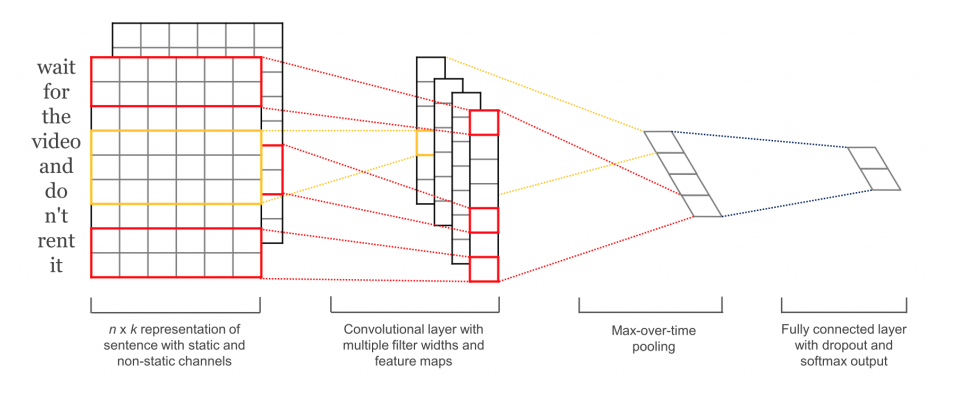
\includegraphics[width=0.5\textwidth]{images/cnn_architecture1.png}

The first layers embeds words into low-dimensional vectors. The next layer performs convolutions over the embedded word vectors using multiple filter sizes. For example, sliding over 3, 4 or 5 words at a time. Next, we max-pool the result of the constitutional layer into a long feature vector, add dropout regularization, and classify the result using a softmax-layer.

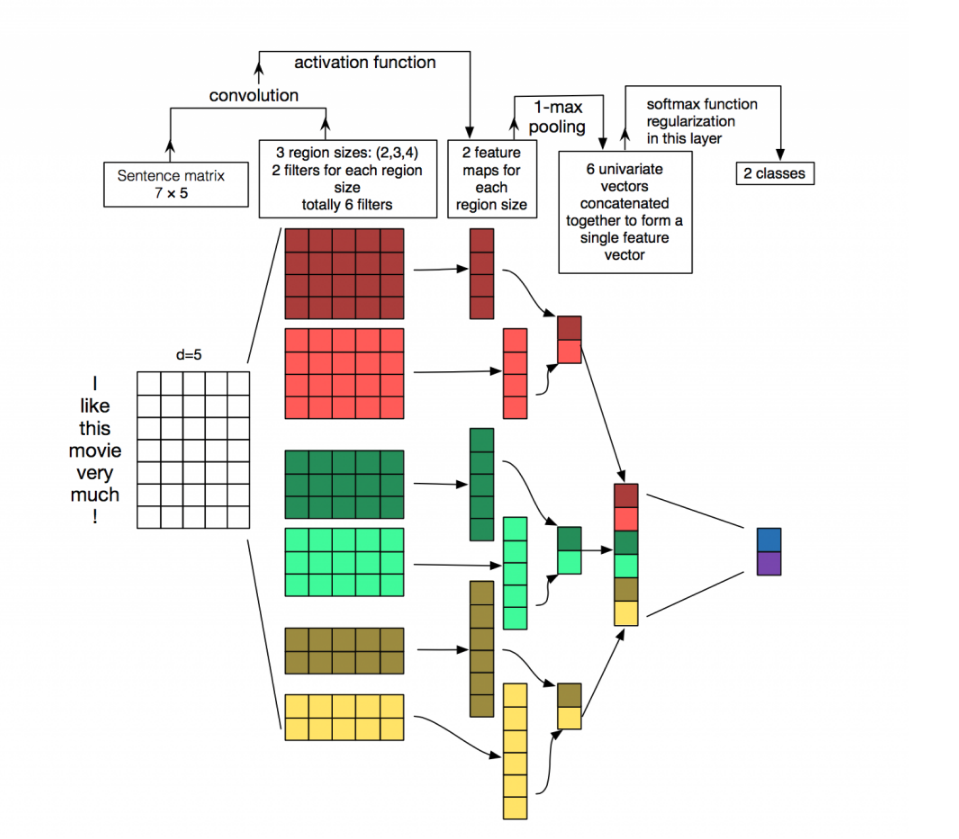
\includegraphics[width=0.5\textwidth]{images/cnn_architecture2.png}

\subsection{Classification Process}

The overall classification process can be sub-divided into two elementary parts:First we feed input data to the neural network to then classifying the (test-)data for their respective classes.

The following steps were taken in order to feed data to the Neural Network:

\begin{enumerate}
\item Seven raw text files are prepared, each containing Tweets for respective parties as collected from Twitter.
\item The dataset is then cleaned and tokenized for building a vocabulary.
\item Each sentence was padded to a maximum length. We append special $<$PAD$>$ tokens to all other sentences to make their length equal 35 words. Padding sentences to the same length is useful because it allows us to efficiently batch our data since each example in a batch must be of the same length.
\item For feature extraction from twitter data we utilize a pretrained word-embeddings model to represent every word in vector form. We use word-embeddings \cite{DBLP:journals/corr/abs-1301-3781} trained on 200 million German Tweets using 200 dimensional vector representation of each word \cite{cieliebak2017twitter}.  
\item Finally we build a vocabulary based on our collected data and map each word to an integer between 0 and 109933 (the vocabulary size). Each sentence becomes a vector of integers.
\end{enumerate}

For classifying the user Tweets to the correct political party, we then feed the batches of twitter data along with their correct political party one-hot-encoded labels and train the above defined CNN. To optimize the network we use cross entropy loss defined as
\begin{equation}
	H_{y'}(y) = - \sum_{i} y'_{i} \log (y_{i})
\end{equation}
where $y$ is our predicted probability distribution, and $y'$ is the true distribution (the one-hot vector with the true-class party labels). 


\section{Quantitative Analysis}

For a quantitative analysis of the results, every Tweets are taken as sentences and a sentence vector of the same dimension as the word vectors used for training (i.e. 200 dimensional vector) is constructed. In doing so, the Tweet is tokenized into words and every word's corresponding token vectors are taken from the word embedding space. A sentence embedding vector is constructed by adding the word vectors and dividing them by the number of words. Note that only those Tweets for which all its words were present in the word embedding space are considered and that any Tweets with \emph{UNK} token were ignored for a cleaner analysis. This effectively removes any Tweets that were not completely related to political topics such as simple link- or hashtag-forwarding. 

The sentence embedding was used to visualize the vectors based on their 200-dimensional vector representations. The initial results were generally pretty mixed up with no clear distinct clusters for any specific party.

We found several reasons for this:
Since a user Re-Tweets other parties Tweets with his opinions, it could be that subjects get mixed rather quickly across parties.
Another reason for such mixed clusters could be the fact that any collection of party-members is typically tweeting about similar issues with some in favor of and some against some specific proposition, which may lead to strictly disconnected sentiment groups within the same party.

As such, a direct embedding as described earlier did not prove to be a good measure to visualize the result. This motivates our usage of the ``political compass'' \cite{PoliticalCompass} for visualizing the result further. 

For the political compass representation, we use a four way graph plot with attributes of ``Left-wing'' and ``Right-wing'' on the X-axis as well as  ``Authoritarian'' and ``Libertarian'' on the Y-axis. On the four axis, we used a one hot encoding to plot all the seven classes on the compass. This way we can see all the political classes plotted at once.

\subsection{Visualization}

Now, we need to plot all the users on the compass to see which users corresponds to what cluster by:
\begin{enumerate}
	\item Passing all of a user's Tweets to the classification model as specified above in the model architecture section
	\item Obtaining the class classification and probability scoreper Tweet concerning all seven classes
	\item Averaging all probability distribution to get one vector representing the distribution over all classes
	\item Plotting the user on the political compass to visualize the results and to compare whether the user has been classified to it’s correct class.
\end{enumerate}

\subsection{Inference}

The subsequent visualizations have been created as described above.

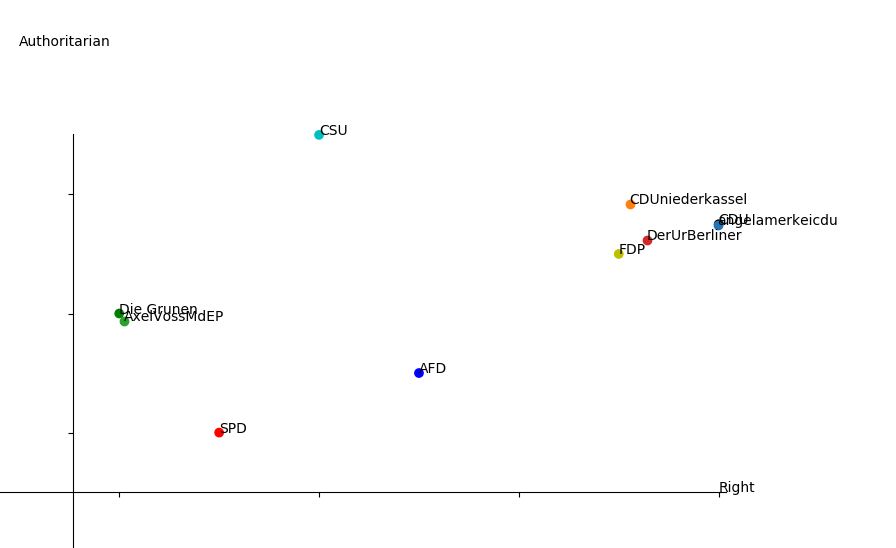
\includegraphics[width=0.5\textwidth]{images/Political_Compass.png}
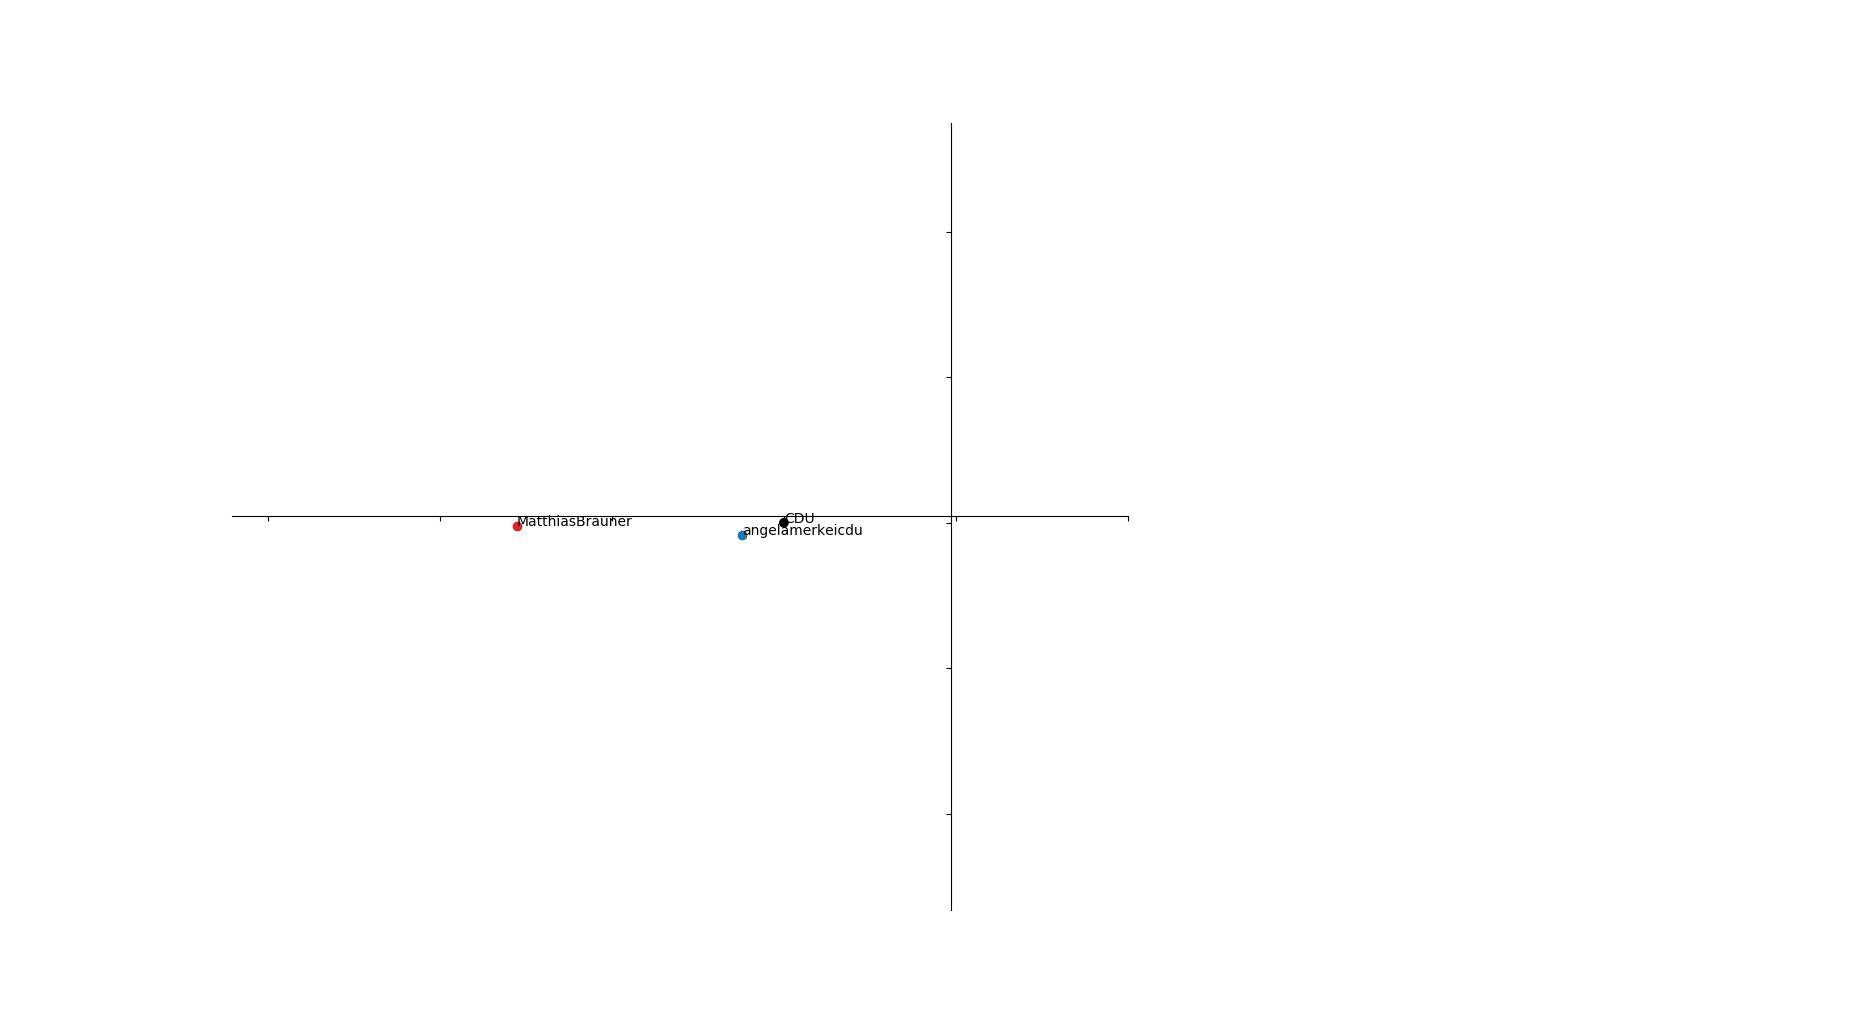
\includegraphics[width=0.5\textwidth]{images/Political_Compass-1.png}

From these visualizations within the political compass, we can derive the following:

\begin{enumerate}
	\item Users generally appear close to their respective political party; e.g. Angela Merkel is very near to CDU
	\item The FDP-class is plotted close to the CDU-class. Both party's ideology are traditionally quite similar, which matches the visualization
	\item The user ``DerUrBerliner'' from the party CDU was found to appear very close to SPD. In out context, this indicates a strong affiliation towards SPD instead of CDU. Upon analyzing the data, we observed a common occurence  of Tweets in the English language, which will have led to a huge number of $<$UNK$>$ token generation, hence the classification may not be correct. After manually cleaning the data, we were able to see the user's plot moving to the correct class CDU.
\end{enumerate}


\section{Conclusion}

As we have shown, a comparably simple convolutional neural network is able to nicely separate political figures concerning party affiliation. Interesting findings like single entities more closely connecting to general party-affiliated language or specifically different language have been pointed out.

As the underlying word embeddings are taken from the German-language Wikipedia dump, we are currently restricted to German-language Tweets as well as to overall German-language features. This does suffice for general classification purposes, but poses the additional question of how the analysis would be affected if the embeddings were to be taken from \emph{intrinsically political} data samples. 
Also, our approach primarily focuses on CNNs and proves them to be efficient already. For future work, it would be intriguing to compare the capabilities of RNNs or other topologically different architectures. 


\end{multicols}

\bibliography{lit}
\bibliographystyle{apalike}

\end{document} 
